%=================================================================
\subsection{Real Data Example}
%=================================================================
\begin{frame}
  \frametitle{Birnbaum-Saunders and Leemis Real Data}
\begin{footnotesize}
\begin{block}{Data I  - from \citeN{Birnbaum/Saunders:1969b} }
\begin{color}{red}
0.07, 0.09, 0.096, 0.097, 0.099, 0.1, 0.103, 0.104, 0.104,
0.105, 0.107, 0.108, 0.108, 0.108, 0.109, 0.109, 0.112, 0.112,
0.113, 0.114, 0.114, 0.114, 0.116, 0.119, 0.12, 0.12, 0.12, 0.121,
0.121, 0.123, 0.124, 0.124, 0.124, 0.124, 0.124, 0.128, 0.128,
0.129, 0.129, 0.13, 0.13, 0.13, 0.131, 0.131, 0.131, 0.131, 0.131,
0.132, 0.132, 0.132, 0.133, 0.134, 0.134, 0.134, 0.134, 0.134,
0.136, 0.136, 0.137, 0.138, 0.138, 0.138, 0.139, 0.139, 0.141,
0.141, 0.142, 0.142, 0.142, 0.142, 0.142, 0.142, 0.144, 0.144,
0.145, 0.146, 0.148, 0.148, 0.149, 0.151, 0.151, 0.152, 0.155,
0.156, 0.157, 0.157, 0.157, 0.157, 0.158, 0.159, 0.162, 0.163,
0.163, 0.164, 0.166, 0.166, 0.168, 0.170, 0.174, 0.196, 0.212
\end{color}
\end{block}

\begin{block}{Data II - Example 8.16 in \citeN{Leemis:1995}}
17.88, 28.92, 33.00, 41.52, 45.12, 45.60, 48.48, 51.84, 51.96,
         54.12, 55.56, 67.80, 68.64, 68.64, 68.88, 84.12, 93.12, 98.64,
        105.12, 105.84, 127.92, 128.04, 173.40
\end{block}
\end{footnotesize}
%----------
\end{frame}

%% %%--------------------------------
\begin{frame}   %%[allowframebreaks]
\begin{figure}[h]
   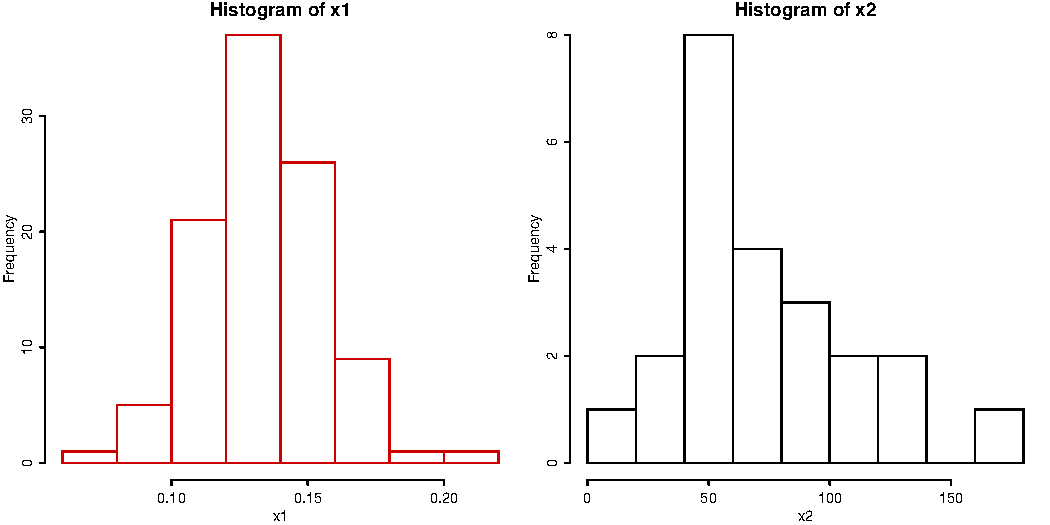
\includegraphics[width=4.5in]{hist4.pdf} %%-Figure (pdf file)
   \vspace{-3ex}
\end{figure}
\end{frame}

%% %%---------------------------------------------------
\begin{frame}   %%[allowframebreaks]
\begin{figure}[h]
   %%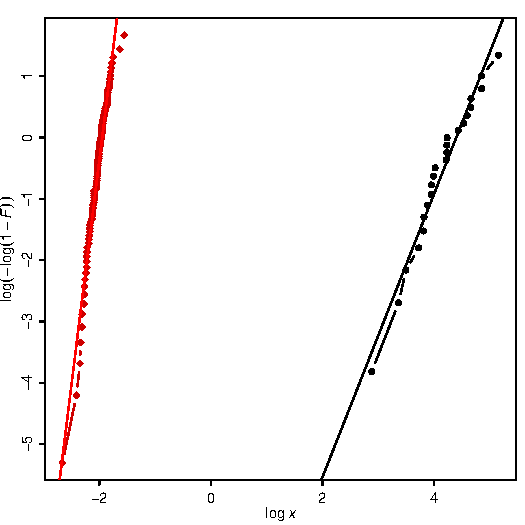
\includegraphics[width=3.0in,angle=90]{Weibull4.pdf} %%-Figure (pdf file)
   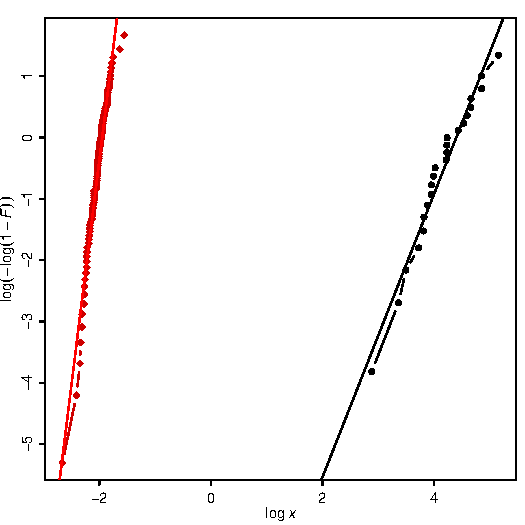
\includegraphics[width=3.0in]{Weibull4.pdf} %%-Figure (pdf file)
   \vspace{-3ex}
\end{figure}
\end{frame}
%% %%---------------------------------------------------



%% %%---------------------------------------------------
\begin{frame}   %%[allowframebreaks]
\begin{block}{How to determine whether the data are from Weibull or not}
\( \qquad
H_0: \text{Weibull}   \mathrm{~~versus~~}   H_1: \text{non-Weibull}  \)
\end{block}
\begin{itemize}
\item Recall: $\log\big\{ -\log(1-p) \big\} = \log\lambda + \alpha \log x_p.$
\item Thus \fbox{$\log\big\{ -\log(1-\hat{p}_i) \big\}$} versus \fbox{$\log x_{(i)}$}
draws a straight line, where $\hat{p}_i= (i-0.375)/(n+0.25)$.
Thus, the linearity measure (sample correlation) can be used for Weibullness test.
\item Idea: Large $r$ implies Weibullness.
\[ \boxed{  H_0: r \ge r_0  \mathrm{~~versus~~} H_1:  r < r_0 } \]
  Then,  how large is large enough for $r$? 
\item To this end, we should know the distribution of $r$ and then find the critical value
(from pivot) with the significance level (or Type-I error).
\end{itemize} 
\end{frame}
%% %%---------------------------------------------------


%% %%---------------------------------------------------
\begin{frame}   %%[allowframebreaks]
\begin{block}{Distribution of \(r\) sample correlations under the normal distribution}
If $(X,Y)$ is from bi-variate normal, it is known that 
\[  r\sqrt{ \frac{n-2}{1-r^2} } \sim t\text{-distribution} \]
with $n-2$ degrees of freedom.
\begin{itemize}
\item In general, $-1 \le r \le 1$, and $ -\infty < r\sqrt{\frac{n-2}{1-r^2}} < \infty$.
\item As $n \to \infty$, CLT works in general. 
      I.e., $r\sqrt{ \frac{n-2}{1-r^2} } \stackrel{d}{\to}N(0,1) $
\item In the Weibull plot,  $ 0 <  r \le 1$. 
      Thus, $0 < r\sqrt{\frac{n-2}{1-r^2}} < \infty$.
\item CLT can not work for the Weibull case.
\end{itemize}
\end{block}\end{frame}
%% %%---------------------------------------------------

%% %%---------------------------------------------------
\begin{frame}   %%[allowframebreaks]
\begin{itemize}
\item We can not use normal approximation. We need to find the distribution of $r$.
\item We can find the distribution of $r$ under Weibull distribution using Monte Carlo simulation. \\
\item Again, recall $\log\big\{ -\log(1-p) \big\} = \log\lambda + \alpha \log x_p.$ \\
\item Since $\mathrm{cor}(aX+b,cY+d) = \mathrm{cor}(X,Y)$, it is enough to generate random sample
of size $n$ from any Weibull distribution.
 This implies that the correlation 
from the Weibull plot is independent of the parameters $\alpha$ and $\lambda$.
\item Thus, the sample correlation is a \textbf{pivotal quantity}.
\end{itemize}
\end{frame}
%----------
\begin{frame}  
\begin{block}{Algorithm}
\begin{itemize}
\item Generate Weibull random observations of size $n$ from any Weibull, say, Weibull (1,1).
\item Sort the data. Denote $x_{(i)}$.
\item Calculate $\log\big\{ -\log(1-\hat{p}_i) \big\}$ where $\hat{p}_i= (i-0.375)/(n+0.25)$.
\item Calculate the sample correlation between $\log\big\{ -\log(1-\hat{p}_i) \big\}$ and $\log x_{(i)}$.
\item Repeat the above (say, up to $N$ iteration numbers).
\item Find the empirical quantiles for critical values (say, 5\%, 10\%, etc.)
\end{itemize}
\end{block}\end{frame}




%% %%---------------------------------------------------
\begin{frame}   %%[allowframebreaks]
\begin{figure}[h]
   %%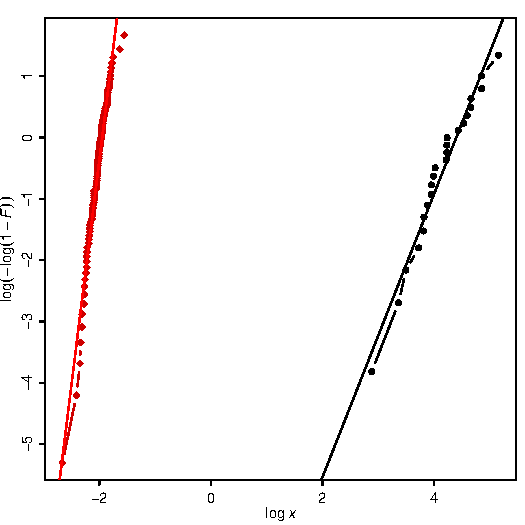
\includegraphics[width=3.0in,angle=90]{Weibull4.pdf} %%-Figure (pdf file)
   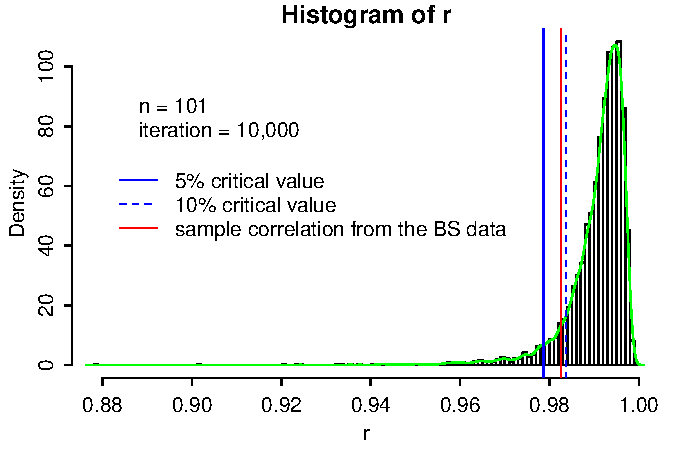
\includegraphics[width=4.5in]{hist-corr1.pdf} %%-Figure (pdf file)
   \vspace{-3ex}
\end{figure}
\end{frame}
%% %%---------------------------------------------------



%% %%---------------------------------------------------
\begin{frame}   %%[allowframebreaks]
\begin{figure}[h]
   %%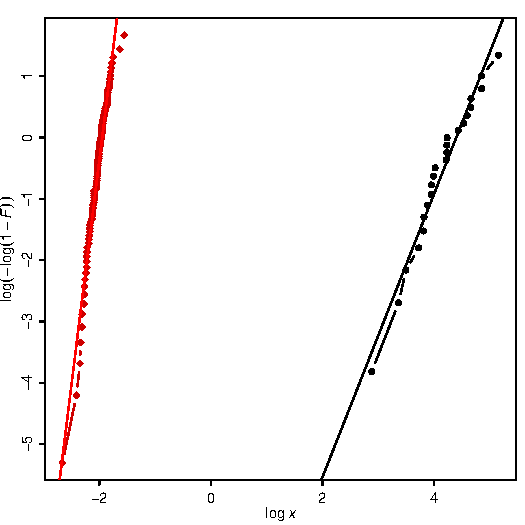
\includegraphics[width=3.0in,angle=90]{Weibull4.pdf} %%-Figure (pdf file)
   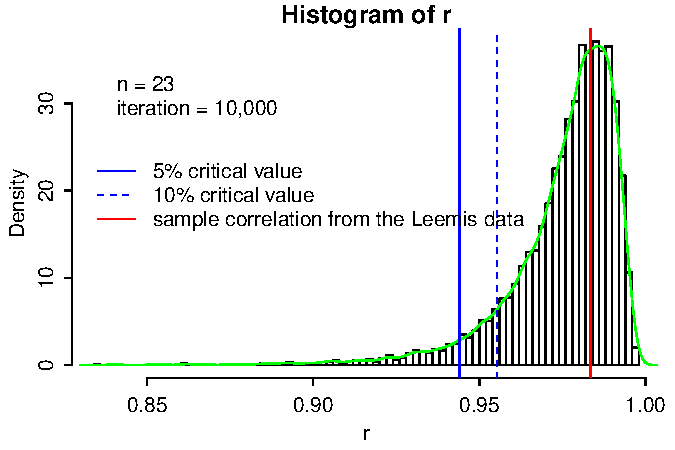
\includegraphics[width=4.5in]{hist-corr2.pdf} %%-Figure (pdf file)
   \vspace{-3ex}
\end{figure}
\end{frame}
%% %%---------------------------------------------------






%% %%---------------------------------------------------
\begin{frame}   %%[allowframebreaks]
\begin{block}{Critical Values}
\begin{tabular}{cccccccc}
\hline
$n$ & &1.0\%  &2.0\%  &2.5\%  &5.0\%  &10\%   &20\%  \\
\hline
101 & &0.9593 &0.9686 &0.9710 &\textcolor{red}{0.9777} & \textcolor{red}{0.9833} &0.9878 \\
 23 & &0.9085 &0.9239 &0.9284 &0.9429 &0.9553 &0.9665 \\
\hline
\end{tabular}
\end{block}

\begin{block}{Sample Correlations for the BS and Leemis Data Sets}
\begin{itemize}
\item Data I (BS Data) \\
$r = \textcolor{red}{0.982614}$ with $n=101$ \\
Using 5\% Type-I error, the Data are from Weibull.
With 10\% or more Type-I error, the Data are not from Weibull.
\item Data II (Leemis Data) \\
$r = 0.983456$ with $n=23$ \\
The Data are from Weibull for any above Type-I errors.
\end{itemize}
\end{block}
We can also find the $p$-value from the empirical pdf.
The $p$-value for the BS data is 8.5\% while that for the Leemis is 63\%.
\end{frame}
%% %%---------------------------------------------------


%% %%---------------------------------------------------
\begin{frame}   %%[allowframebreaks]
\begin{figure}[h]
   %%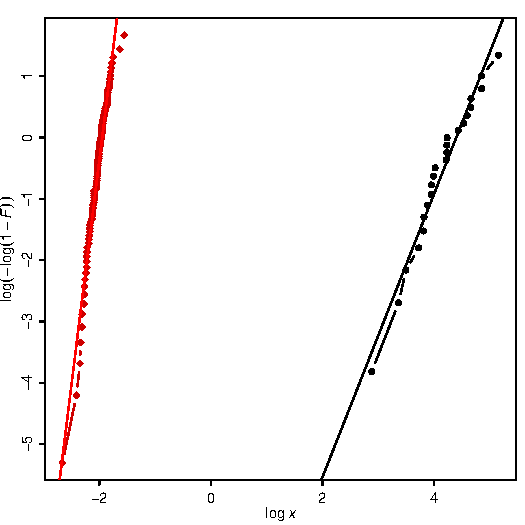
\includegraphics[width=3.0in,angle=90]{Weibull4.pdf} %%-Figure (pdf file)
   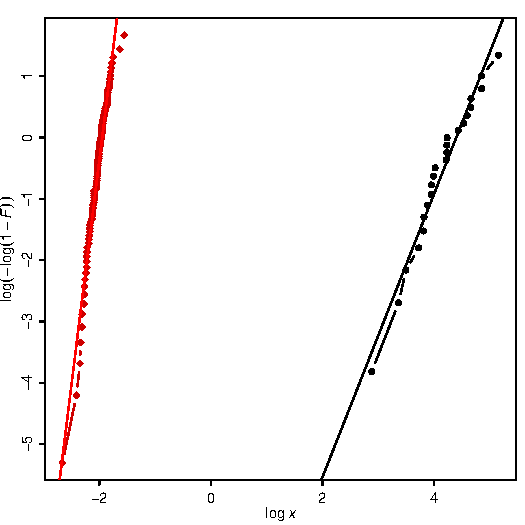
\includegraphics[width=3.0in]{Weibull4.pdf} %%-Figure (pdf file)
   \vspace{-3ex}
\end{figure}
\end{frame}
%% %%---------------------------------------------------


%=================================================================
\subsection{Weibullness R Package}
%=================================================================
%% %%---------------------------------------------------
\begin{frame}[fragile]{Weibullness R Package}
Testing Weibullness can be easily performed by using \texttt{weibullness} R package
\cite{Park:2018b}. 
One can refer to:
\begin{itemize}
\item \url{https://appliedstat.github.io/R/R-package-1/}  \\
     \href{https://appliedstat.github.io/R/R-package-1/}{\beamergotobutton{Link}}
\item \url{https://cran.r-project.org/web/packages/weibullness/}  \\
     \href{https://cran.r-project.org/web/packages/weibullness/}{\beamergotobutton{Link}}
\end{itemize}
\begin{exampleblock}{Installation}
\begin{verbatim}
> install.packages("weibullness")

> library("weibullness")
> help(package="weibullness")
\end{verbatim}
\end{exampleblock}
\end{frame}

